\section{Results \label{sec:results}}

The following results are split into three main sections. We firstly present solutions to the LTE using Rayleigh friction and compare dissipation between the analytical and numerical solutions in section \ref{subsec:result_rayleigh}. Section \ref{subsec:result_bottom} then presents purely numerical results for dissipation using only bottom friction. Finally, dissipation in the bottom friction case is compared to analytical scaling laws derived by \citet{chen2013tidal} in section \ref{subsec:scaling}.

\subsection{Rayleigh Friction \label{subsec:result_rayleigh}}
\begin{figure*}[!t]
\begin{subfigure}{\linewidth}
\centering
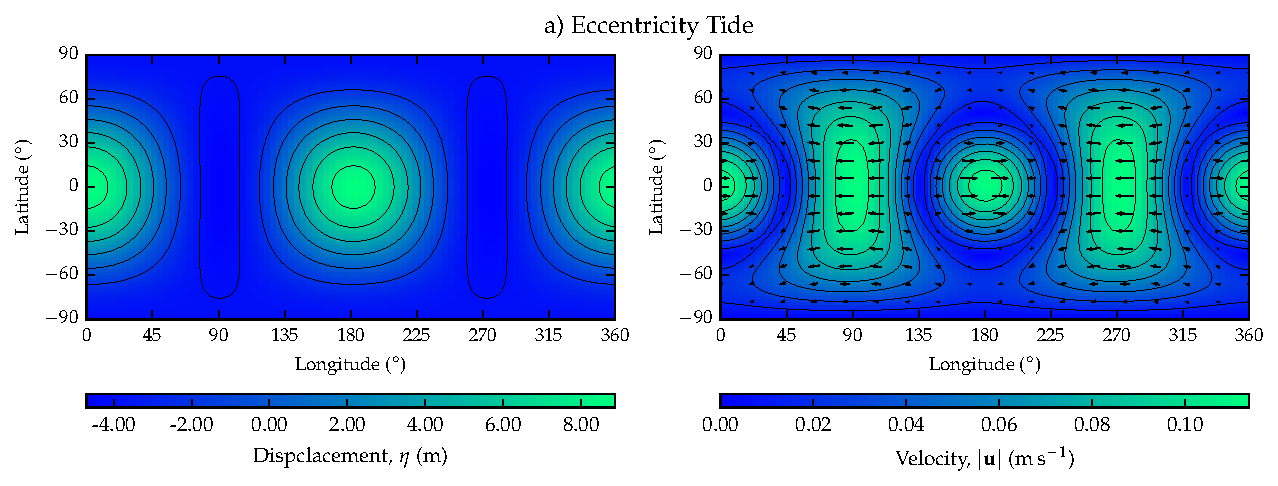
\includegraphics[width=0.8\linewidth,trim={0 0 0 0.2cm},clip]{Figures/Ecc_test}
\subcaption{\label{fig:LTE_a}}
\end{subfigure}\vspace*{-0.7cm}
\begin{subfigure}{\linewidth}
\centering
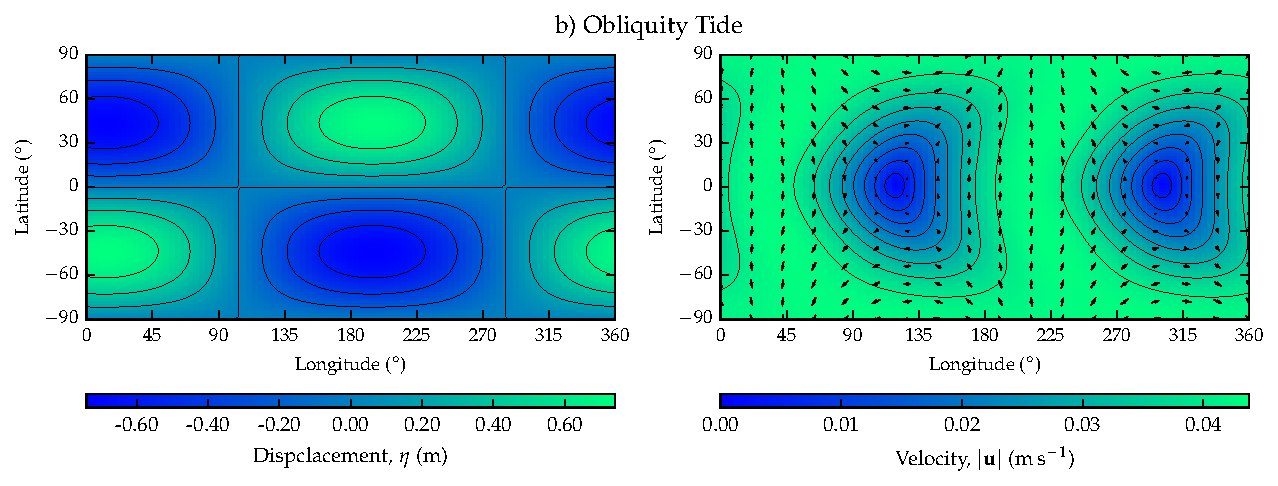
\includegraphics[width=0.8\linewidth]{Figures/Obliq_test}
\subcaption{\label{fig:LTE_b}}
\end{subfigure}\vspace*{-0.7cm}
\begin{subfigure}{\linewidth}
\centering
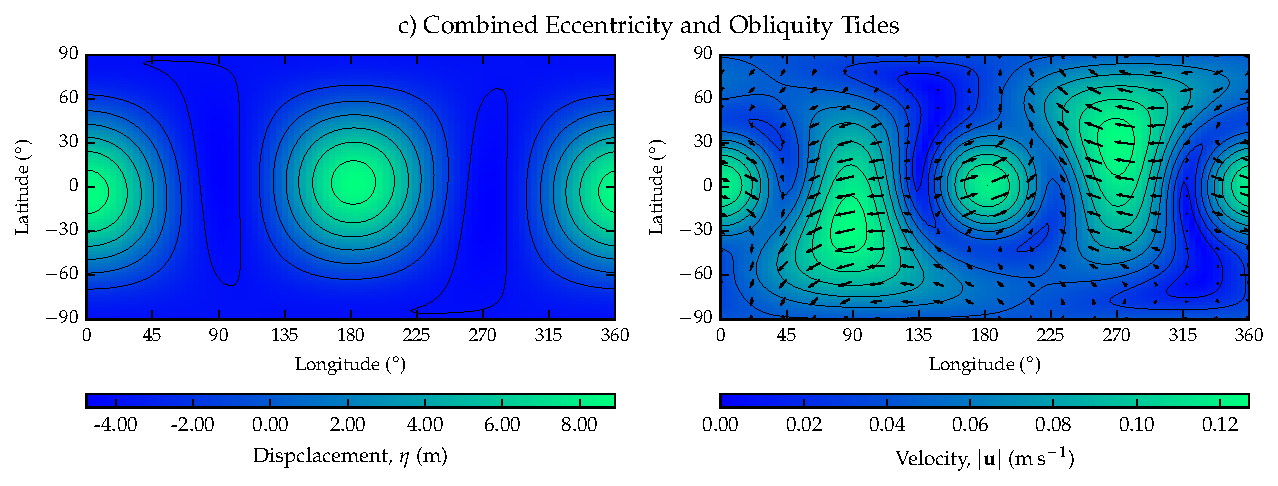
\includegraphics[width=0.8\linewidth]{Figures/Full_test}
\subcaption{\label{fig:LTE_c}}
\end{subfigure}\vspace*{-0.8cm}
\caption{Solutions to the LTE under the eccentricity (eq. \ref{eq:U_ecc}), obliquity (eq. \ref{eq:U_obliq}), and full tidal potential (eq. \ref{eq:U_2}). $h = 400 \, \si{\metre}$ and $\alpha = 2.28 \times 10^{-7} \, \si{\per\second}$ in a), b) and c).\label{fig:LTE_solns}}
\end{figure*}

The primary task of ODIS is to solve the LTE on a sphere, and it is from these solutions that dissipation is derived. Thus, a useful starting point is to illustrate the actual solutions to the LTE rather than purely concerning the reader with the average tidal dissipation over an orbital period. 

Figure \ref{fig:LTE_solns} illustrates numerical solutions to the LTE at periapse for different components of the tidal potential. Surface displacement, $\eta$, is illustrated on the left, whereas velocity, $\bm{u}$, is on the right. The colour scale in the velocity figures represents the velocity's magnitude, $\left| \bm{u} \right|$, Arrows indicate the direction of flow. The tidal forcing applied is, from a) to c), the eccentricity tide, obliquity tide, and both tides combined together, respectively. All plots are for the ``canonical'' $400 \, \si{\metre}$ ocean outlined by \citet{sagan1982tide} to allow best comparison with \citet{sears1994tidal,sears1995tidal,sohl1995tidal}. The coefficient of Rayleigh friction is maintained at $\alpha = 2.28 \times 10^{-7} \, \si{\per\second}$, as mentioned in section \ref{subsec:param}.

Surface displacement in Figure \ref{fig:LTE_a} illustrates a classic tidal bulge, centered on the Saturnian ($\phi = 0^{\circ}$) and sub-Saturian ($\phi = 180^{\circ}$) points. Maximum displacement is over $8$ metres. Away from the tidal bulge displacement drops below the equilibrium level to less than $4$ metres. The corresponding flow pattern shows convergence and divergence at the longitudinal positions of steepest gradient in the displacement field, whereas the fastest flow occurs in the most shallow displacement gradients.

The obliquity tide shows markedly different displacement and flow patterns than the eccentricity tide (Figure \ref{fig:LTE_b}). Displacement is now anti-symmetric about the equator. Notably, the longitudinal positions of maxima and minima are offset from the Saturnian and sub-Saturnian points. The tide raised by the obliquity tidal potential is also an order of magnitude less than the eccentricity tide. Flow is mainly poleward, converging south of the equator on the Saturn-facing hemisphere, and north of the equator on the opposite hemisphere.

The final plot in figure \ref{fig:LTE_solns} is the solution under the full tidal potential. In many ways, it is similar to the eccentricity tide. Yet, the addition of the obliquity tide adds significant equatorial asymmetry to the solutions. This asymmetry is particularly noticeable in the velocity plot on the right hand side of Figure \ref{fig:LTE_c}, where the areas of fastest flow are skewed north and south of the equator, unlike in Figure \ref{fig:LTE_a}. This is also evident in the displacement field, where the tidal bulge maximum does not lie directly on the equator.

Comparisons made between the results in Figure \ref{fig:LTE_solns} and the analytical solutions show excellent agreement for this test case.

The simulations used in Figure \ref{fig:LTE_solns} were run from undisturbed initial conditions: \hbox{$\eta = 0 \, \si{\metre}$} and \hbox{$\bm{u} = (0,0) \, \si{\metre\per\second}$}. Consequently, there is some start-up time required for the model to converge into its periodic equilibrium, as described by \citet{sears1995tidal}. Figure \ref{fig:diss} illustrates this issue. From left to right, the figure shows orbitally averaged dissipation against time for the eccentricity-libration, eccentricity-radial, and obliquity tides.  The solid lines represent the average dissipation over each orbit in the numerical model, while the dashed lines indicate the analytical time-averaged dissipation value. 

\begin{figure}[!t]
\centering
\begin{subfigure}{\linewidth}
\centering
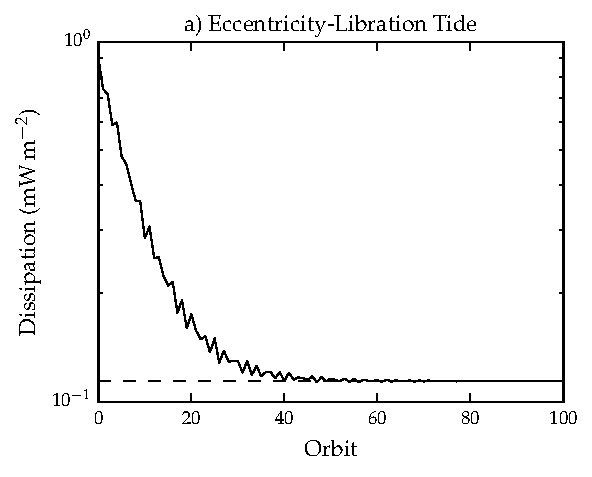
\includegraphics[width=0.8\linewidth]{Figures/ecc_lib_diss}
\subcaption{\label{fig:diss_a}}
\end{subfigure}\vspace*{-0.7cm}
\begin{subfigure}{\linewidth}
\centering
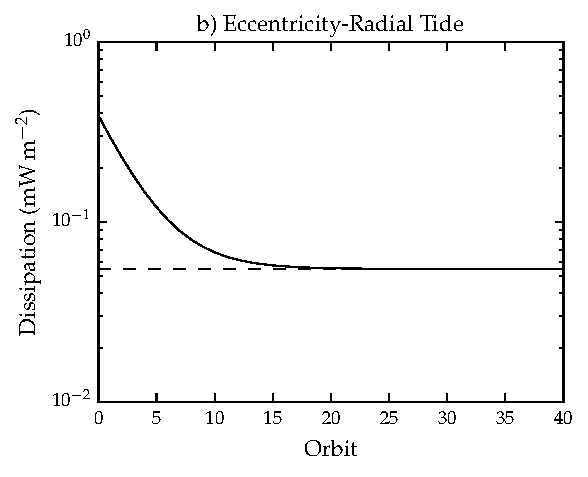
\includegraphics[width=0.8\linewidth]{Figures/ecc_rad_diss}
\subcaption{\label{fig:diss_b}}
\end{subfigure}\vspace*{-0.7cm}
\begin{subfigure}{\linewidth}
\centering
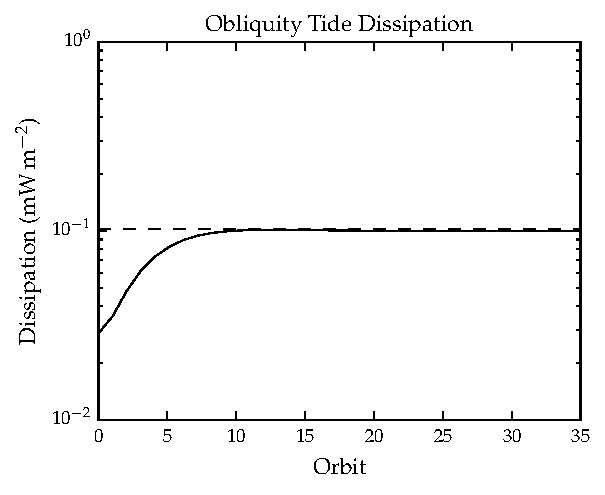
\includegraphics[width=0.8\linewidth]{Figures/obliq_diss}
\subcaption{\label{fig:diss_c}}
\end{subfigure}
\vspace*{-0.8cm}
\caption{Average dissipation over each orbit under the eccentricity (eq. \ref{eq:U_ecc}), obliquity (eq. \ref{eq:U_obliq}), and full tidal potential (eq. \ref{eq:U_2}). $h = 400 \, \si{\metre}$ and $\alpha = 2.28 \times 10^{-7} \, \si{\per\second}$.\label{fig:diss}}
\end{figure}




\subsection{Bottom Friction \label{subsec:result_bottom}}

\subsection{Scaling Laws \label{subsec:scaling}}